\begin{frame}{Triangle excercise}
\begin{enumerate}
\item Sides AB and AC of $\triangle$ABC are extended to points P and Q respectively.Also,$\angle$PBC $<$ $\angle$QCB.Show that AC$>$AB .
\begin{center}
%Code by GVV Sharma
%December 6, 2019
%released under GNU GPL
%Drawing a right angled triangle

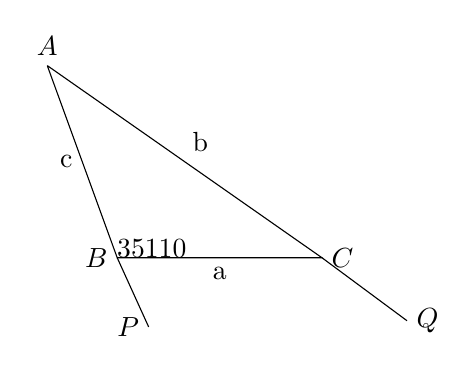
\begin{tikzpicture}[scale=0.4]

%Triangle sides
\def\a{6.5}
\def\c{6.5}
\def\b{10.64}

%Marking coordiantes
\coordinate [label=above:$A$] (A) at (-2.22,6.10);
\coordinate [label=left:$B$] (B) at (0,0);
\coordinate [label=right:$C$] (C) at (6.5,0);
\coordinate [label=left:$P$] (P) at (1,-2.2);
\coordinate [label=right:$Q$] (Q) at (9.2,-2);

%Drawing triangle ABC
\draw (A) -- node[left] {$\textrm{c}$} (B) -- node[below] {$\textrm{a}$} (C) -- node[above,,xshift=2mm] {$\textrm{b}$} (A);\draw (B)--(P);
\draw (C)--(Q);
%Drawing and marking angles
\tkzMarkAngle[arc=l,size=1,color=black](A,C,B)
\tkzLabelAngle[pos=1.5](A,C,B){\rotatebox{360}{$35$}}

\tkzMarkAngle[fill=white!40,size=0.5cm,mark=](C,B,A)
\tkzLabelAngle[pos=1](C,B,A){\rotatebox{-360}{$110$}}

\end{tikzpicture}


\end{center}
\end{enumerate}
\begin{itemize}
\item a= 4,b=4.58,c=4
\item cos(C)=-$\frac{c^2 - b^2 -a^2}{2ab}$
\item cos(C)=55

\seti
\end{itemize}
\end{frame}
\begin{frame}
\begin{center}
\begin{figure}
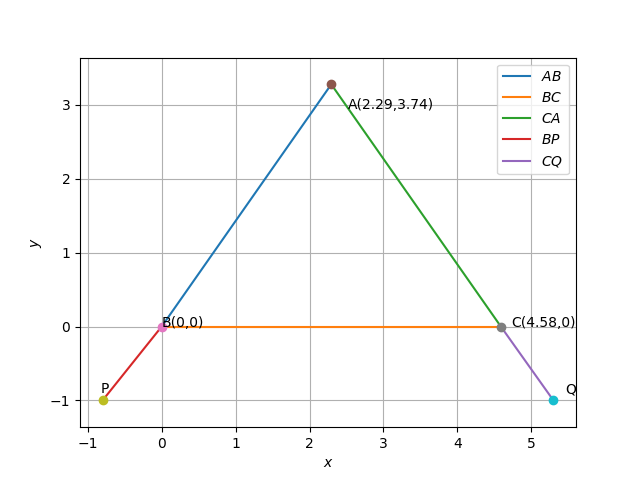
\includegraphics[scale=.4]{./CODES/triangle/tri_ex.png}
\end{figure}
\end{center}
\begin{itemize}
\item \url{https://github.com/pratibha444/GEOMETRY/blob/master/figs/TRI_EX.tex}
\item \url{https://github.com/pratibha444/GEOMETRY/blob/master/CODES/triangle/TRIANGLE_EXCERCISE.py}
\end{itemize}
\end{frame}



\begin{frame}
\begin{itemize}

\item \textbf{Given} : P and Q are extended to AB and AC respectively.\\
And $\angle$PBC $<$ $\angle$QCB --(1)\\
So,\\
$\angle$PBC + $\angle$ABC = 180$\degree$  \\
$\angle$QCB + $\angle$ACB = 180$\degree$  \\
\end{itemize}
$\angle$PBC = 180 - $\angle$ABC --(2)\\
$\angle$QCB = 180 - $\angle$ACB --(3)\\
By substituting the value of $\angle$PBC and $\angle$QCB in equation 1 \\
180 - $\angle$ABC $<$ 180 - $\angle$ACB\\
-$\angle$ABC $<$ -$\angle$ACB\\
multiplying both the sides by '-'\\
-(-$\angle$ABC) $>$  -(-$\angle$ACB)\\
$\angle$ABC $>$ $\angle$ACB   (sides opposite to greater angle is longer)\\
\end{frame}